\documentclass[runningheads]{llncs}
\usepackage{amsmath}
\usepackage{amssymb}
\usepackage{tikz}
\usetikzlibrary{shapes}
\tikzset{
circ/.style={draw,circle,minimum height=3em},
}

\begin{document}

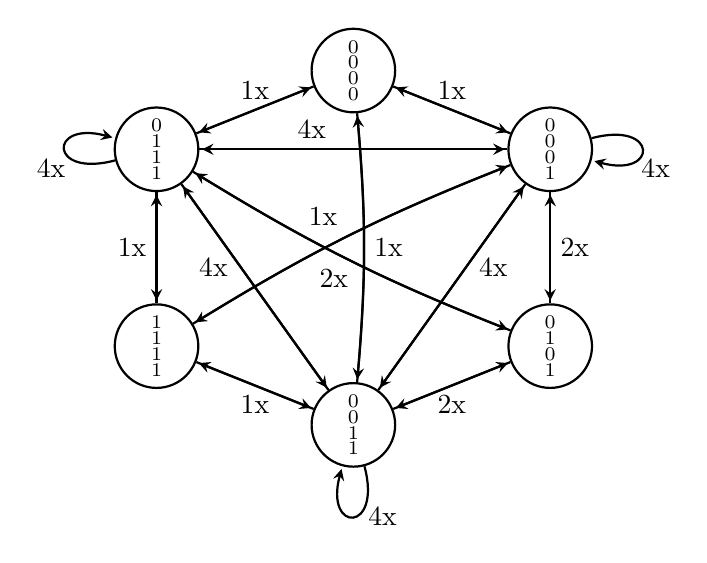
\begin{tikzpicture}[->,>=stealth,shorten >=1pt,auto,node distance=5cm,thick,node/.style={circle,draw}]
  \node[node] at (1.5,3.5) (0111) {$\substack{0\\1\\1\\1}$};
  \node[node] at (4,4.5) (0000) {$\substack{0\\0\\0\\0}$};
  \node[node] at (6.5,3.5) (0001) {$\substack{0\\0\\0\\1}$};
  \node[node] at (1.5,1) (1111) {$\substack{1\\1\\1\\1}$};
  \node[node] at (6.5,1) (0101) {$\substack{0\\1\\0\\1}$};
  \node[node] at (4,0) (0011) {$\substack{0\\0\\1\\1}$};
  \path
    (0111) edge [loop left] node [below] {4x\quad\quad} (0111)
           edge node [above]  {1x} (0000)
           edge node [] {} (1111)
           edge [bend right=5] node {} (0101)
           edge node [above] {4x\quad\quad\quad\quad} (0001)
           edge node [above] {4x\quad\quad\quad\quad} (0011)
    (0001) edge [loop right] node [below] {\quad4x} (0001)
           edge node []  {} (0101)
           edge node [] {} (0000)
           edge [bend right=5] node {} (1111)
           edge node [above] {\quad\quad\quad4x} (0011)
           edge node [] {} (0111)
    (0011) edge [loop below] node [right] {\,4x} (0011)
           edge node []  {} (1111)
           edge node [] {} (0101)
           edge [bend right=5] node {} (0000)
           edge node [] {} (0111)
           edge node [] {} (0001)
    (0000) edge node  [above] {1x}(0001)     
           edge [bend left=5] node {1x} (0011)     
           edge node {} (0111) 
    (0101) edge node [below]  {2x} (0011)     
           edge [bend left=5] node [below] {2x\quad\quad} (0111) 
           edge node [right] {2x} (0001) 
    (1111) edge node [left] {1x} (0111)     
           edge [bend left=5] node {1x} (0001)     
           edge node [below] {1x} (0011); 
\end{tikzpicture}

\end{document}